%%%%%%%%%%%%%%%%%%%%%%%%%%%%%%%%%%%%%%%%%%%%%%%%%%%%%%%%%%%%%%%%%%%%%%%%%%%%%%%%
%2345678901234567890123456789012345678901234567890123456789012345678901234567890
%        1         2         3         4         5         6         7         8

\documentclass[letterpaper, 10 pt, conference]{ieeeconf}  % Comment this line out if you need a4paper

%\documentclass[a4paper, 10pt, conference]{ieeeconf}      % Use this line for a4 paper

\IEEEoverridecommandlockouts                              % This command is only needed if 
                                                          % you want to use the \thanks command

\overrideIEEEmargins                                      % Needed to meet printer requirements.

%In case you encounter the following error:
%Error 1010 The PDF file may be corrupt (unable to open PDF file) OR
%Error 1000 An error occurred while parsing a contents stream. Unable to analyze the PDF file.
%This is a known problem with pdfLaTeX conversion filter. The file cannot be opened with acrobat reader
%Please use one of the alternatives below to circumvent this error by uncommenting one or the other
%\pdfobjcompresslevel=0
%\pdfminorversion=4

% See the \addtolength command later in the file to balance the column lengths
% on the last page of the document

% The following packages can be found on http:\\www.ctan.org
\usepackage{graphics} % for pdf, bitmapped graphics files
\usepackage{graphicx} % 用于包含图形
\usepackage{epsfig} % for postscript graphics files
\usepackage{mathptmx} % assumes new font selection scheme installed
\usepackage{times} % assumes new font selection scheme installed
\usepackage{amsmath} % assumes amsmath package installed
\usepackage{amssymb}  % assumes amsmath package installed
\usepackage{algorithm}      % 提供算法浮动体（带标题、编号、引用）
\usepackage{algpseudocode}  % 提供伪代码语法（if/for/while/函数等）
\usepackage{booktabs} % for \toprule, \midrule, \bottomrule
\usepackage[caption=false,font=footnotesize]{subfig}
\usepackage{cite}

% 导入 geometry 宏包
\usepackage[
  % a4paper,                % 纸张大小
  left=19.1mm,              % 左边距
  right=19.1mm,             % 右边距
  top=19.1mm,               % 上边距
  bottom=19.1mm,            % 下边距
  % headheight=15pt,        % 页眉高度
  % footskip=10mm           % 页码到正文底部的距离
]{geometry}


\title{\LARGE \bf
Remember Your Driving Feel: Proprioception Based Online Learning for UGV Traversability Across Complex Terrains
}


% \author{Zikang Xie$^{1\dagger}$, Binhan Du$^{1\dagger}$, Kexin Fei$^{1}$, Shucheng Li$^{1}$, Zhenping Sun$^{1}$, Xiaohui Li$^{1}$, Dewen Hu$^{1}$, and Jian Li$^{1*}$
\author{\small Zikang Xie$^{1\dagger}$, Binhan Du$^{1\dagger}$, Kexin Fei$^{1}$, Shucheng Li$^{1}$, Zhenping Sun$^{1}$, Xiaohui Li$^{1}$, Dewen Hu$^{1}$, and Jian Li$^{1*}$
\thanks{$^{\dagger}$These authors contributed equally to this work.}% <-this % stops a space
\thanks{$^{*}$Corresponding author}% <-this % stops a space
\thanks{$^{1}$All authors are with the College of Intelligence Science and Technology, National University of Defense Technology, China. 
        {\tt\small lijian@nudt.edu.cn}}%
}


\begin{document}



\maketitle

\thispagestyle{empty}
\pagestyle{empty}




%%%%%%%%%%%%%%%%%%%%%%%%%%%%%%%%%%%%%%%%%%%%%%%%%%%%%%%%%%%%%%%%%%%%%%%%%%%%%%%%
\begin{abstract}

Robust navigation in complex unstructured environments remains a critical challenge for Unmanned Ground Vehicles (UGVs). Conventional exteroceptive perception methods relying on LiDAR and cameras are inadequate to characterize actual traversability, often resulting in risky situations or navigation failures. For example, icy or waterlogged roads are geometrically flat but prone to wheel slippage, whereas grass clumps visually appear as obstacles yet are safely traversable. The core limitation is that geometric profiles and rigid semantic labels cannot capture the inherent mechanical properties of terrains, and the exteroceptive perception paradigm fails to bridge the gap from visual appearance to embodied understanding. To address this, inspired by human cognitive mechanisms, we propose Proprioception-based Online Learning for UGV Traversability (\textit{POLT}). This framework enables the online learning and prediction of complex terrain traversability through proprioceptive feedback and dynamic memory. Specifically, a Temporal-aware Physics-Informed Neural Network (T-PINN) is designed to learn traversability from real-time proprioceptive signals. Meanwhile, a dynamic memory mechanism is introduced to fuse offline physical priors with online experiences for knowledge accumulation and fast adaptation. Experiments demonstrate that our method  outperforms both exteroceptive perception-based and online learning-based baselines, and it can learn and predict terrain traversability adaptively across the challenging road conditions of icy, waterlogged and grass clump-covered terrains.

\end{abstract}

%%%%%%%%%%%%%%%%%%%%%%%%%%%%%%%%%%%%%%%%%%%%%%%%%%%%%%%%%%%%%%%%%%%%%%%%%%%%%%%%
\section{INTRODUCTION}

With the rapid advancement of sensor technology and deep learning, the environmental perception capabilities of UGVs have achieved remarkable progress. Existing perception methods leverage LiDAR and cameras to accomplish high-precision geometric reconstruction and semantic segmentation, thereby building detailed 3D environmental maps \cite{c1, c2}. However, relying solely on traditional perception is far from sufficient in complex unstructured environments. The system must bridge the gap from ``observation" to ``understanding" for achieving truly intelligent autonomous navigation, which requires accurately inferring the complex physical interactions between the terrain and the vehicle platform.

This gap between visual appearance and physical reality is ubiquitous in the real world \cite{c3, c4}, as shown in Fig. 1. Taking the example of icy roads, the terrain is geometrically flat but suffers a drastic drop in friction, making the vehicle susceptible to slippage. Meanwhile, in grass-covered areas, grass clumps visually resemble solid obstacles and are erroneously avoided despite being physically traversable, leading to overly conservative navigation or even mission stagnation. In contrast, human drivers do not rely solely on ``eyes'' under complex ground conditions. They achieve robust driving through the deep integration of visual anticipation and proprioceptive feedback \cite{c5, c6}. On icy segments, drivers reduce their speed when they sense the ``wheels are not gripping the road'', indicating tire slippage; similarly, in off-road environments, they rely on vehicle vibration feedback to assess the traversability of grass clumps. This inconsistency between exteroception and proprioception demonstrates that relying solely on external perception or rigid offline priors has fundamental limitations in dynamic, unknown, and unstructured environments \cite{c7, c8}.


% 放在右栏顶部的单栏图片
\begin{figure}[t]
  \centering
  % 宽度设为 0.48\textwidth 以适应单栏宽度并留出微小边距
  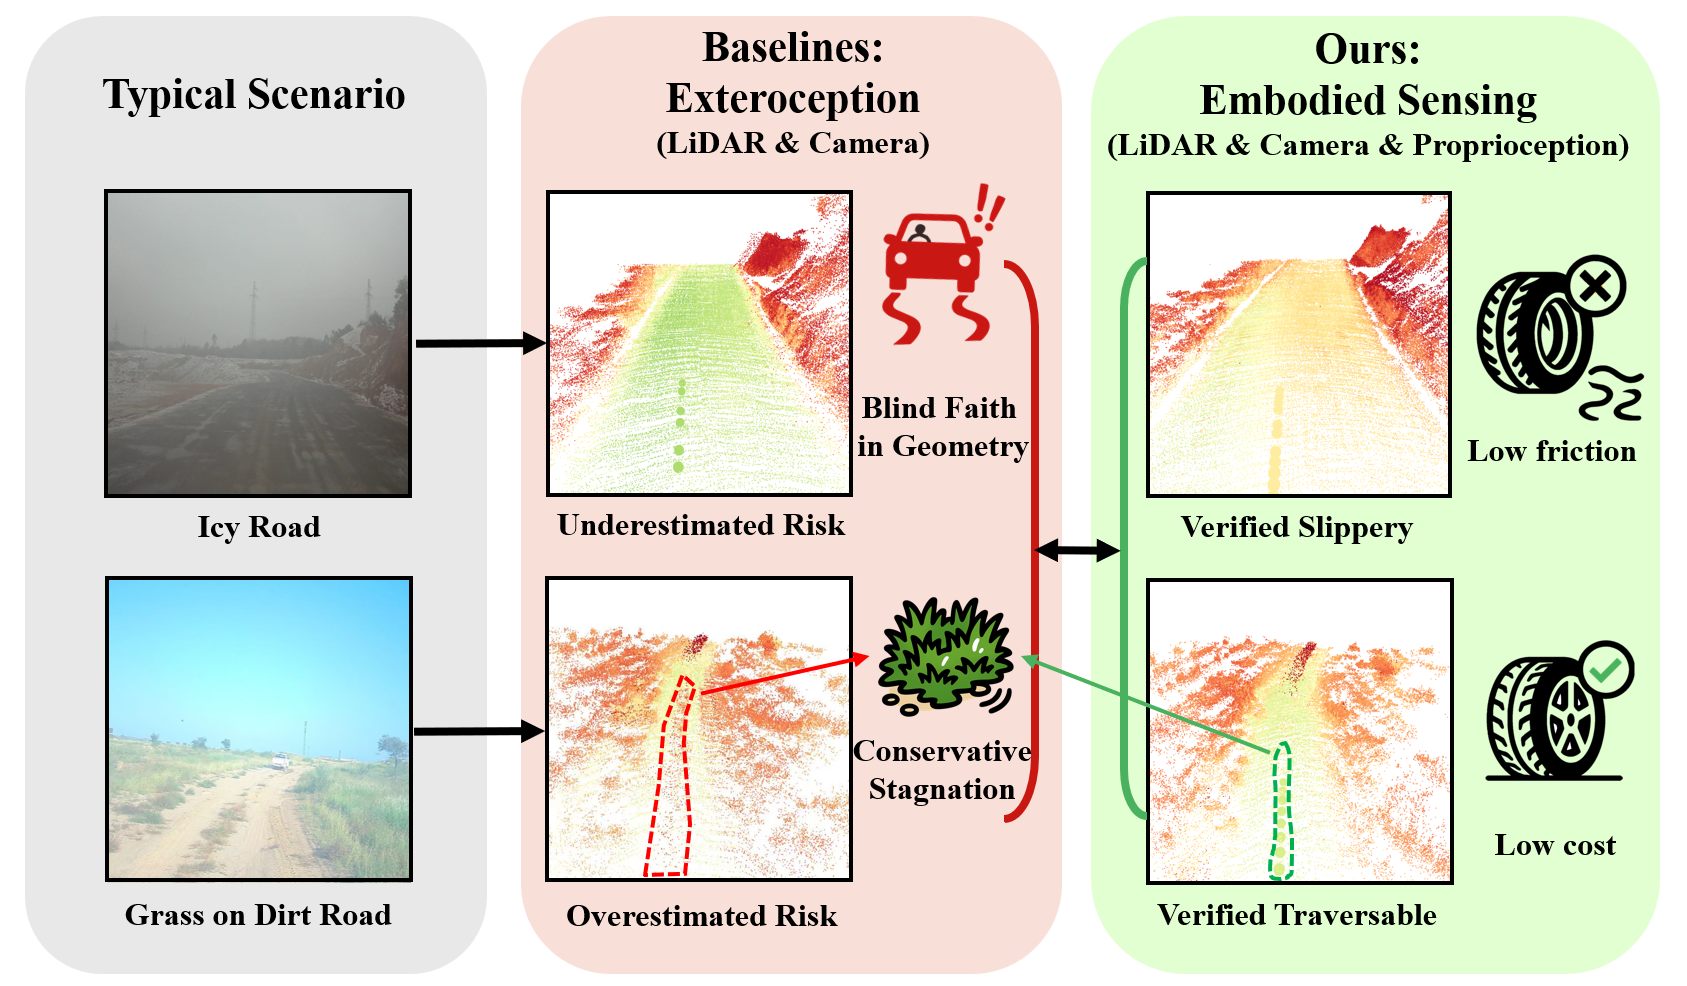
\includegraphics[width=0.48\textwidth]{images/fig_1.png}
  \caption{Motivation of our embodied sensing: (Top) Icy roads are geometrically flat but slippery, leading to underestimated risk in exteroception. (Bottom) Grass clumps are often misclassified as obstacles, causing conservative navigation. Our method utilizes proprioceptive feedback to resolve these ambiguities.}
  \label{fig:motivation_single_column}
\end{figure}

\begin{figure*}[t]
% \vspace*{2mm} % <--- 加入这行
    \centering
    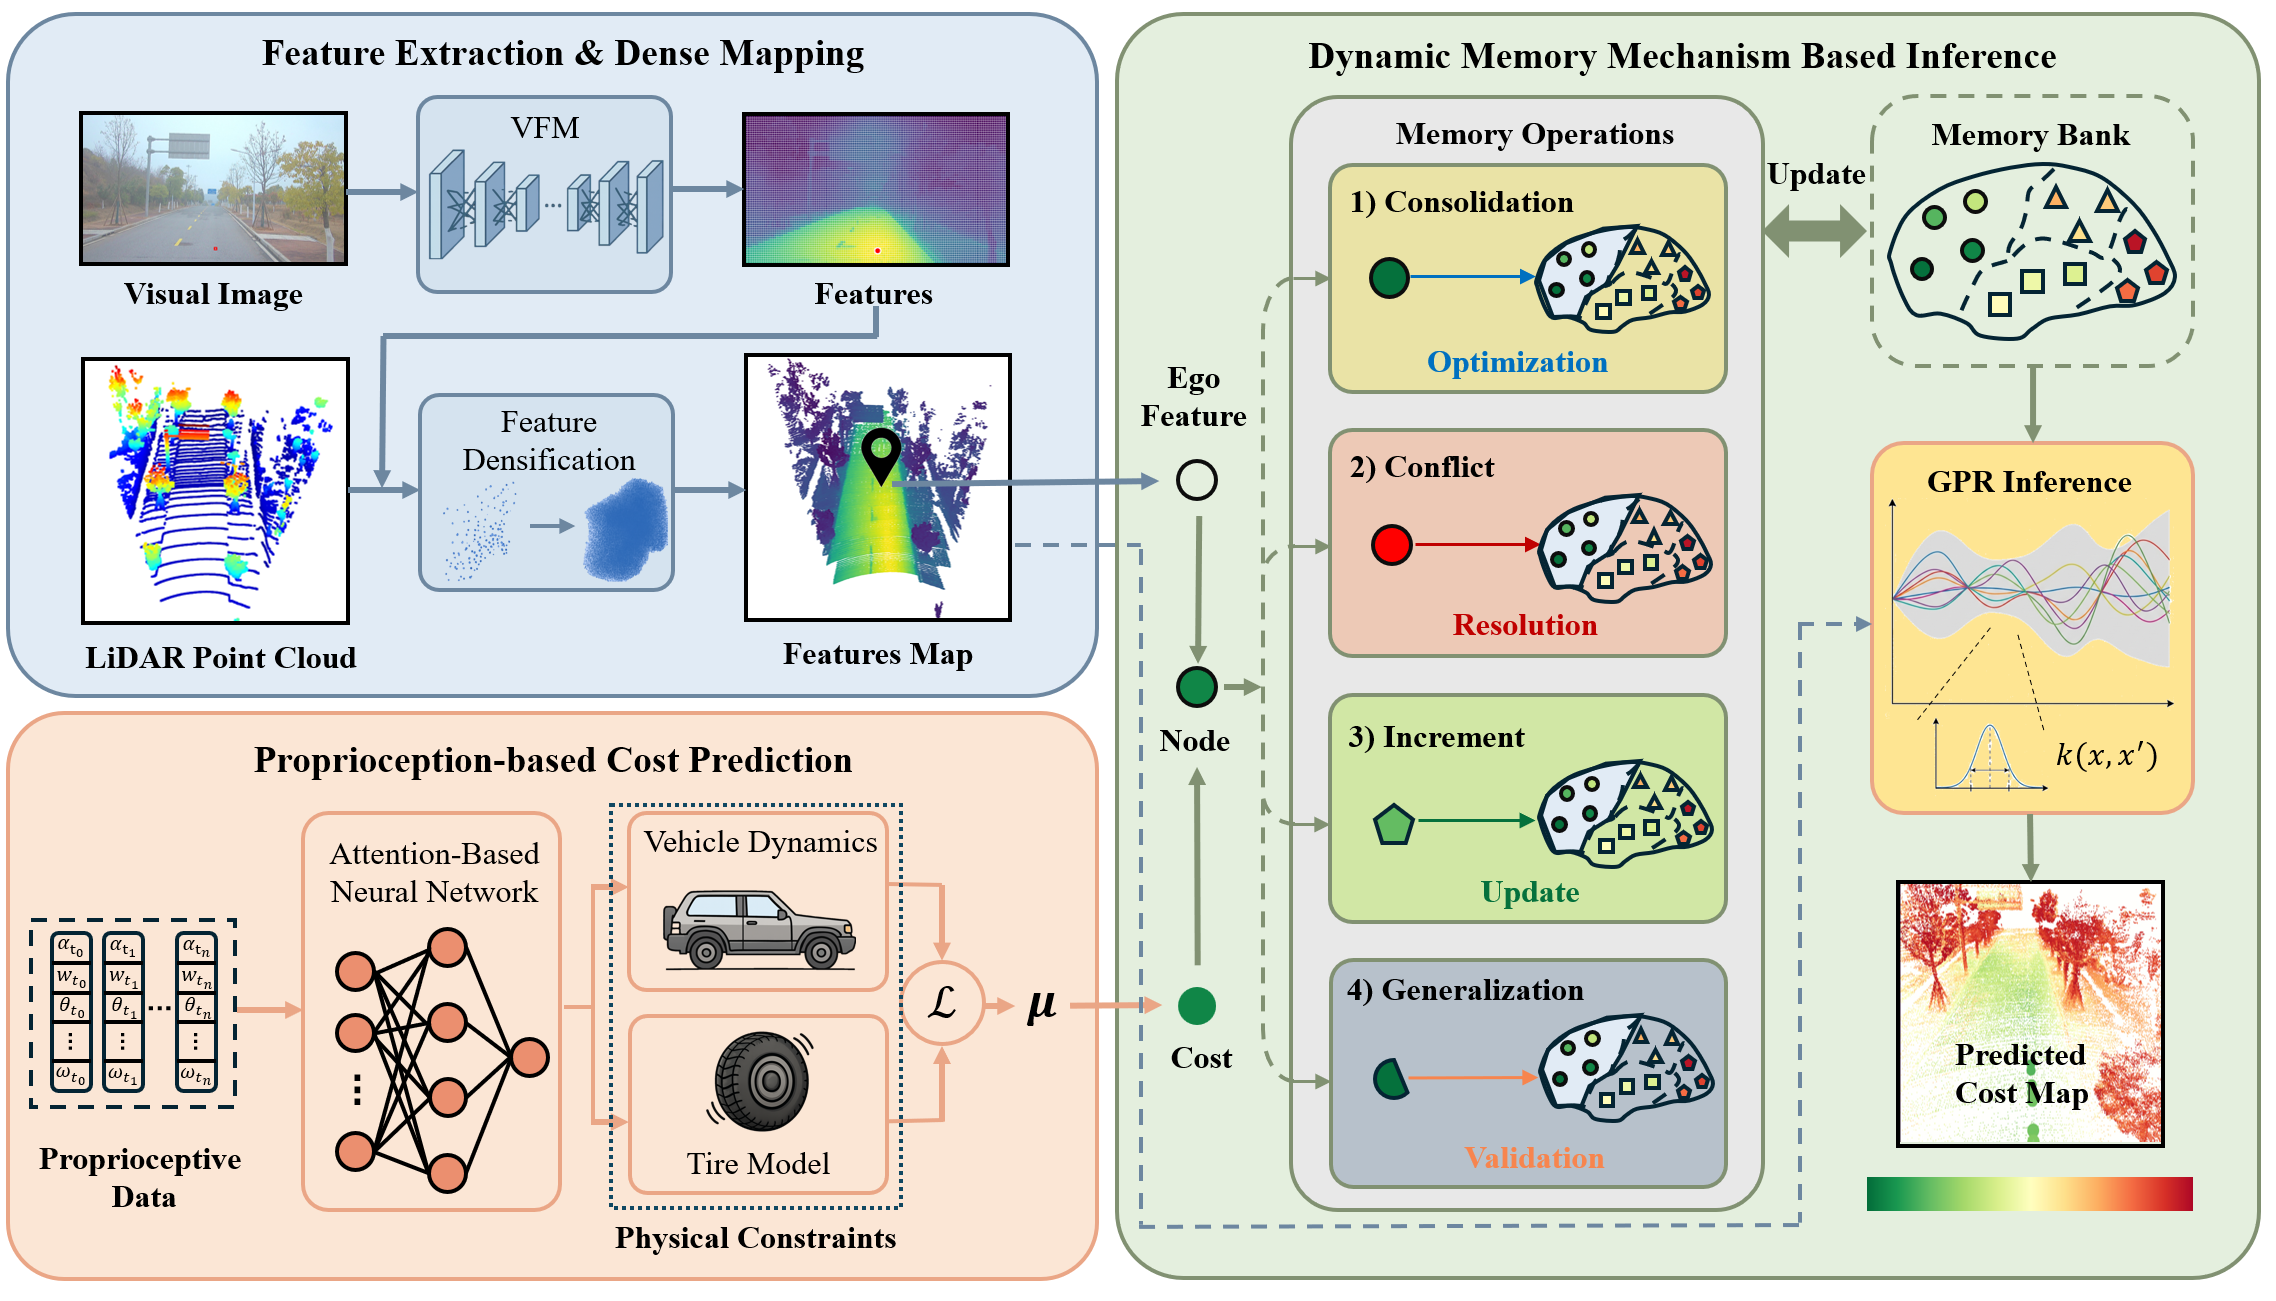
\includegraphics[width=\textwidth]{images/fig_2.png}
    \caption{Overall architecture of the proposed method. The system integrates exteroceptive feature mapping (top), physics-informed proprioceptive cost prediction via T-PINN (bottom-left), and a dynamic memory mechanism based on Gaussian Process Regression (right), which  enables robust, real-time adaptation to complex terrains.}
    \label{fig:architecture}
\end{figure*}

To break through this bottleneck, the UGV navigation paradigm urgently needs to shift from exteroception to embodied proprioception \cite{c9, c10}. Whereas exteroceptive perception aims to construct static geometric and semantic maps, proprioception serves as the dynamic bridge connecting environmental appearance to the UGV's traversability cost \cite{c11}. This embodied mechanism endows the UGV with a proprioceptive intuition akin to that of a human driver, enabling it to dynamically calibrate the deviations of visual priors based on real-time interactive feedback.

Inspired by human cognitive mechanisms, we propose Proprioception-based Online Learning for UGV Traversability (\textit{POLT}). It integrates proprioceptive feedback with exteroceptive perception to analyze and predict traversability, while accumulating driving experience via a dynamic memory mechanism. Just as a human explorer senses ground slipperiness through their footsteps to evaluate the path ahead, \textit{POLT} utilizes real-time proprioception as a feedback signal to unveil the true mechanical properties of the terrain. It then leverages visual similarity to extrapolate this localized physical feedback into global traversability predictions. Furthermore, to emulate the human ability to consolidate experience, we construct a dynamic memory mechanism that inherits offline physical priors and actively updates obsolete knowledge based on real-time interactions. Consequently, instantaneous embodied perception is adaptively transformed into robust, long-term navigational experience.

In summary, our main contributions are as follows:
\begin{itemize}
\item \textbf{\textit{POLT}, an embodied traversability analysis and prediction method fusing proprioception and online memory:} It utilizes proprioceptive feedback to learn the mechanical properties of the currently traversed terrain, and extrapolates this localized knowledge to predict the traversability of the area ahead.
\item \textbf{A dynamic memory mechanism capable of fusing offline priors with online proprioception:} It achieves rapid adaptation to unknown terrains and continuous knowledge accumulation through the strategy of offline experience guidance and online scene updating.
\item \textbf{Extensive experimental validation:} Comprehensive evaluations across diverse challenging terrains (e.g., snow, mud, and grass clumps) demonstrate that \textit{POLT} significantly outperforms existing exteroceptive and online learning baselines in terms of environmental understanding and prediction accuracy.
\end{itemize}


\section{RELATED WORKS}

\subsection{Traversability analysis}

Traversability analysis aims to establish a mapping from exteroceptive sensor data to terrain traversability cost. Conventional exteroceptive perception methods predominantly rely on vision and LiDAR for environmental perception. LiDAR-based approaches typically quantify terrain using grid-based elevation maps or statistical point cloud features \cite{c12, c13, c14}; however, the reliability of these methods severely degrades in adverse weather conditions, such as rain, fog, or dust. Vision-based techniques, including recent visual foundation models, leverage semantic segmentation or zero-shot feature extraction to classify terrain categories (e.g., grass, gravel) as proxies for physical properties \cite{c15, c16, c17, c18}. Nonetheless, relying strictly on visual appearance often leads to perceptual ambiguities in complex off-road environments. To mitigate single-modality limitations, multi-modal fusion strategies align LiDAR geometry with visual or spectral data to construct joint geometric-semantic representations for enhanced scene understanding \cite{c19, c20, c21}. Despite these advancements, such offline-trained models are inherently bounded by their static training distributions, leading to a drastic drop in generalization capability when deployed in unknown or dynamic off-road scenarios.

\subsection{Proprioception}

Proprioception enables a vehicle to infer external environmental properties through its internal kinematic and dynamic states. Early research in this domain originated with planetary rovers, utilizing terramechanics and wheel-soil interaction models to evaluate the bearing capacity and sinkage risk of soft terrains \cite{c22, c23}. In legged robotics, tactile sensors and joint encoders are widely used to capture contact forces and motion impedance, providing direct observations of terrain physical properties \cite{c24, c25, c26}. As UGVs transition from structured roads to unstructured off-road environments, traversability assessment has evolved from binary obstacle detection to continuous cost modeling. Proprioception has garnered significant attention in this context, as it inherently encodes terrain mechanical responses and directly reflects the physical deformation induced by vehicle-terrain interactions \cite{c27}. Mainstream UGV approaches utilize Inertial Measurement Units (IMUs) to capture traversal vibrations, quantifying terrain roughness by integrating the power spectral density of vertical accelerations \cite{c8, c9, c10, c28, c29, c30}. However, these statistical features primarily capture geometric undulations and struggle to characterize core terramechanical properties, such as friction coefficients and shear strength. Recent studies have introduced vehicle dynamics modeling and deeply fused visual appearance with proprioceptive feedback, deriving physically consistent traversability metrics through inverse tire-terrain dynamics and parameter identification \cite{c7, c31, c32}.

\subsection{Online Learning}

Online learning addresses concept drift by dynamically adapting to real-time data distribution shifts. Core mechanisms typically involve maintaining a dynamic training buffer for continuous model fine-tuning or employing sliding windows to discard obsolete samples, thereby preserving environmental adaptability. In off-road navigation, this paradigm has been widely adopted for self-supervised traversability analysis, utilizing preceding vehicle trajectories, multi-view cues, or proprioceptive feedback as supervisory signals for online adaptation \cite{c10, c33, c34, c35, c36, c37}. However, existing approaches predominantly rely on First-In-First-Out (FIFO) or maximum-similarity replacement strategies for experience management. Such unstructured memory lacks a semantic evaluation of sample value. Consequently, it fails to resolve the perceptual ambiguity of ``visually similar but mechanically conflicting" terrains and struggles to retain sparse yet critical historical experiences over the long term, ultimately exacerbating catastrophic forgetting. Inspired by the memory architectures of Large Language Model (LLM) agents, recent studies have transitioned from mere data storage to hierarchical cognitive simulation \cite{c38, c39, c40}. In this study, we introduce this structured ``retrieve-reflect-update'' cognitive architecture into physical-world perception. By constructing a dynamic memory mechanism based on Gaussian Process Regression, our method achieves robust prediction of terrain mechanical properties and enables continuous, life-long knowledge accumulation.


\section{APPROACH}

The overall pipeline of the proposed method is illustrated in Fig. \ref{fig:architecture}. \textit{POLT} consists of three core modules: feature extraction and mapping, proprioception-based traversability cost prediction, and online learning integrated with a dynamic memory mechanism. By fusing proprioceptive feedback with exteroceptive representations, our method leverages visual similarities to generalize local traversability cost to the entire terrain.

\subsection{Feature Extraction and Dense Mapping}

We extract robust features via a visual foundation model and project them into 3D using LiDAR-camera calibration and odometry, constructing a dense feature space representation.

\textbf{1) Feature Extraction and Dimensionality Reduction:} To capture the physical properties of off-road scenes without manual annotations, we employ the self-supervised DINOv3 \cite{c41} to map the input RGB image $I_t \in \mathbb{R}^{H \times W \times 3}$ into a dense feature map $\mathbf{F}_t \in \mathbb{R}^{H \times W \times D}$. For efficient online inference, we introduce a VLAD-inspired compression strategy. High-dimensional features $\mathbf{f}_{u,v}$ are distilled into compact descriptors $\mathbf{z}_{u,v}$ via an anchor codebook $\mathcal{C} = \{ \mathbf{c}_1, \dots, \mathbf{c}_K \}$, where the $k$-th element represents the manifold distance:

\begin{equation}
\label{eq:projection}
\mathbf{z}_{u,v}^{(k)} = \| \mathbf{f}_{u,v} - \mathbf{c}_k \|_1
\end{equation}

\textbf{2) 2D-3D Feature Projection and Dense Mapping:} To align 2D visual features with 3D space, we employ a two-stage projection and densification strategy.

\begin{itemize}
\item \textbf{Single-Frame Construction:} For a given feature map and LiDAR point cloud $\mathcal{P}_t$, the projected pixel coordinates $\mathbf{u}_i$ of any 3D point $\mathbf{p}_i$ are:

\begin{equation}
\label{eq:densification}
s \cdot \tilde{\mathbf{u}}_i = \mathbf{K} \cdot \mathbf{T}_{L \to C} \cdot \tilde{\mathbf{p}}_i
\end{equation}

where $\mathbf{K}$ and $\mathbf{T}_{L \to C} \in SE(3)$ denote the camera intrinsics and extrinsics. Bilinear interpolation then assigns a feature descriptor to each spatial point, yielding a single-frame feature point cloud $\mathcal{F}_t$.

\item \textbf{Spatiotemporal Densification:} To mitigate point cloud sparsity in distant regions, we accumulate historical frames within a sliding window $\mathcal{W}$ via LiDAR odometry. Using the relative pose $\mathbf{T}_{t-k}^{t}$, we construct a dense local feature map $\mathcal{M}_t$:

\begin{equation}
\label{eq:manifold_dist}
\mathcal{M}_t = \bigcup_{k=0}^{|\mathcal{W}|} \left\{ (\mathbf{T}_{t-k}^{t} \cdot \mathbf{p}_j, \mathbf{f}_j) \mid (\mathbf{p}_j, \mathbf{f}_j) \in \mathcal{F}_{t-k} \right\}
\end{equation}


\end{itemize}


% 放在右栏顶部的单栏图片
\begin{figure}[t]
% \vspace*{2mm} % <--- 加入这行
  \centering
  % 宽度设为 0.48\textwidth 以适应单栏宽度并留出微小边距
  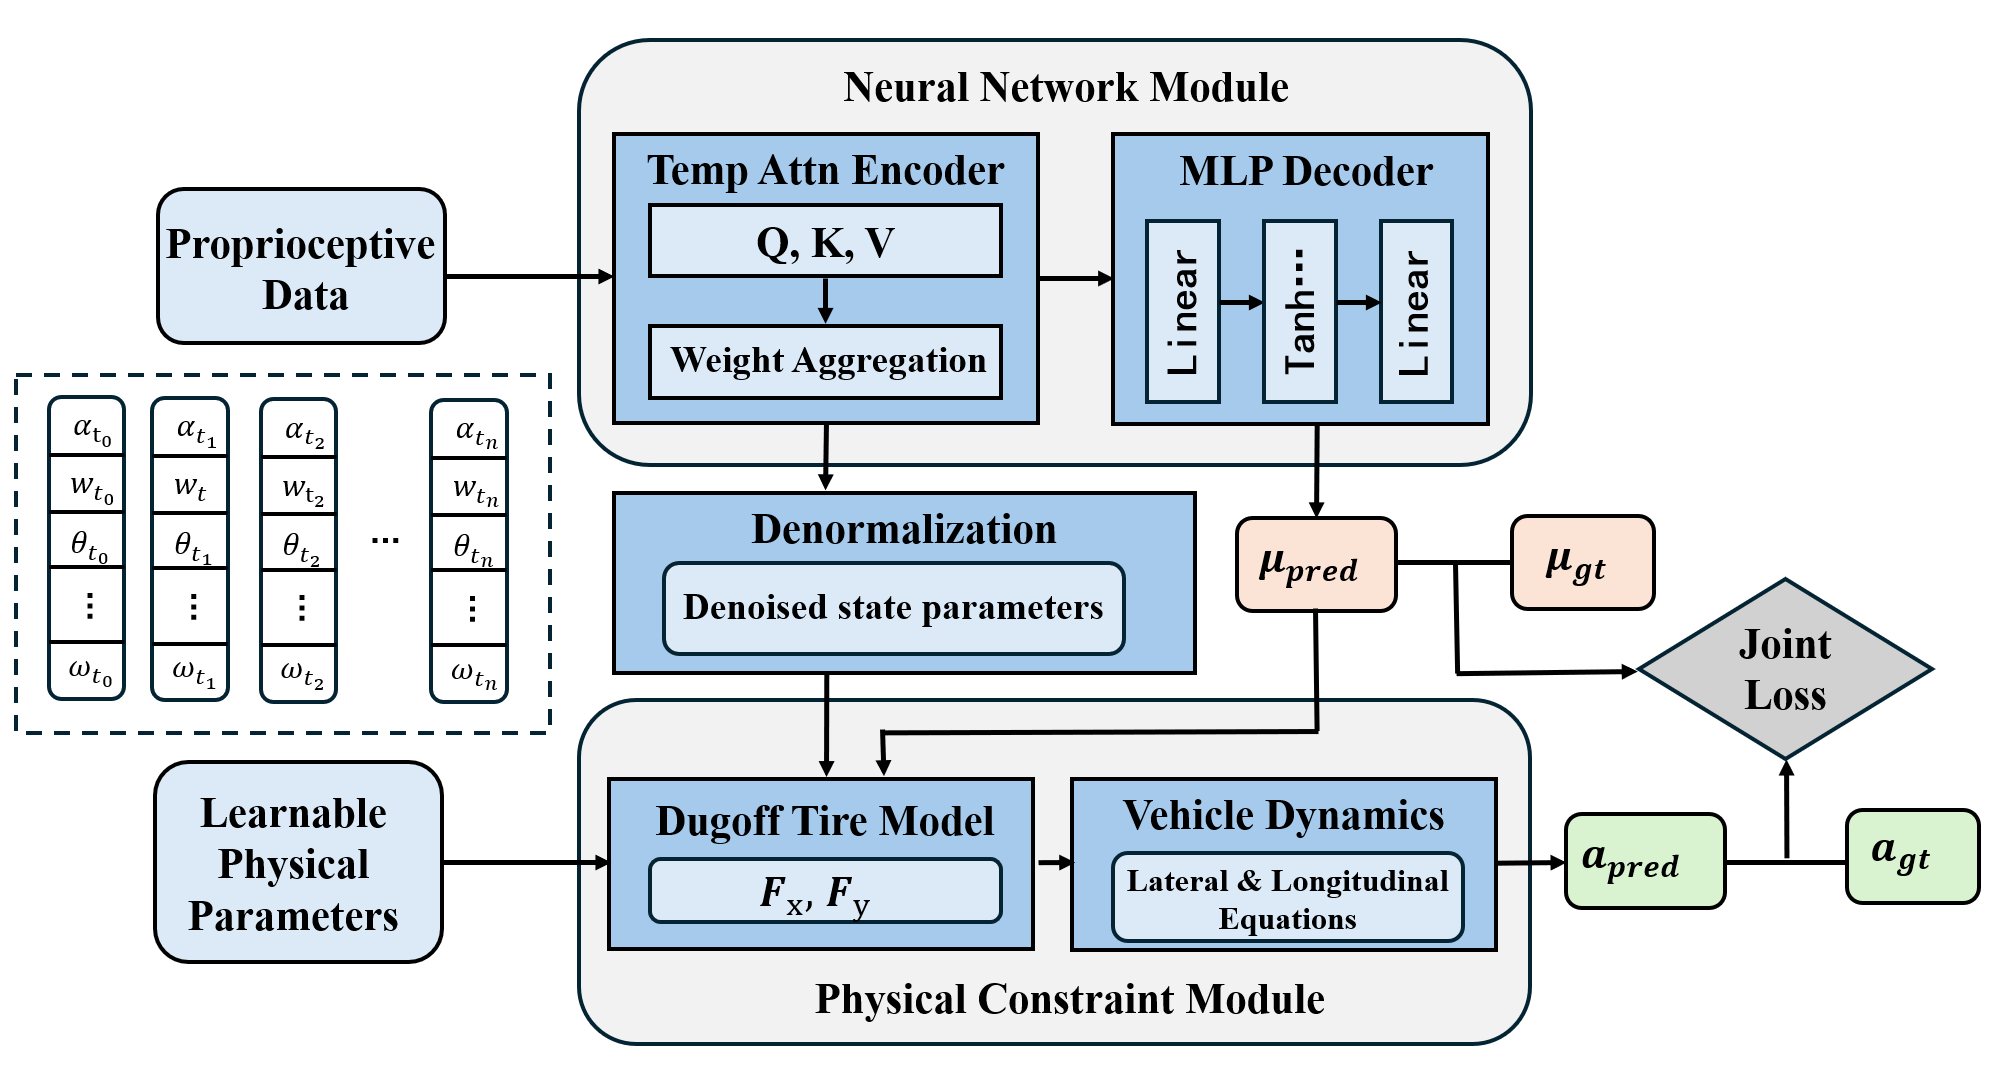
\includegraphics[width=0.48\textwidth]{images/fig_3.png}
  \caption{Structure of the T-PINN. The model utilizes an attention-based encoder to extract denoised state parameters from high-frequency proprioceptive data. A differentiable vehicle dynamics model (Dugoff tire model) acts as a physical consistency constraint, enabling the adaptive online learning of terrain friction coefficients and robust traversability cost prediction.}
  \label{fig:tpinn}
\end{figure}


\subsection{Proprioception-based Traversability Cost Prediction}

To accurately estimate the terrain friction coefficient $\mu$, we propose a Temporal-aware Physics-Informed Neural Network (T-PINN), as detailed in Fig. 3. This architecture integrates data-driven learning with physical constraints: the neural network extracts robust state representations from noisy observations, while differentiable vehicle dynamics restrict predictions to a feasible physical domain.

\textbf{1) Neural Network Module:} To suppress high-frequency noise in off-road sensor data, we employ an attention-based encoder-decoder architecture. The encoder aggregates the historical sequence $\mathbf{X} \in \mathbb{R}^{T \times F}$ into a denoised state vector $\mathbf{h} = \sum_{t=1}^{T} \alpha_t \mathbf{v}_t$ via scaled dot-product attention, providing a robust motion representation for physical residual calculation. An MLP decoder with Tanh activation then maps $\mathbf{h}$ to the predicted friction coefficient $\hat{\mu} = \Phi_{dec}(\mathbf{h}; \mathbf{W}_{net})$.



\textbf{2) Physical Consistency Constraints:} To ensure outputs conform to Newtonian mechanics, vehicle dynamics equations are embedded as regularization terms. Accounting for significant off-road terrain variations, we formulate a dynamics model with slope $\theta$ and roll $\phi$ corrections:


\begin{equation}
\label{eq:vehicle_dynamics}
\left\{
\begin{aligned}
M (a_x - g\sin\theta) &= \sum F_{x,ij} \cos\delta - \sum F_{y,ij} \sin\delta \\
M (a_y - g\sin\phi) &= \sum F_{x,ij} \sin\delta + \sum F_{y,ij} \cos\delta
\end{aligned}
\right.
\end{equation}

where $M$ denotes the vehicle mass; $a_x$ and $a_y$ are the longitudinal and lateral accelerations, respectively; $g$ is the gravitational acceleration; $F_{x,ij}$ and $F_{y,ij}$ represent the longitudinal and lateral tire forces at each wheel; and $\delta$ is the steering angle.


The Dugoff tire model characterizes the nonlinear transition from elastic to sliding regions via a decay factor $f(\lambda)$:

\begin{equation}
\label{eq:dugoff}
\begin{aligned}
f(\lambda) &= \begin{cases} (2-\lambda)\lambda, & \lambda < 1 \\ 1, & \lambda \geq 1 \end{cases} \\
\lambda &= \frac{\mu F_z (1+s)}{2 \sqrt{(C_x s)^2 + (C_y \tan \alpha)^2}}
\end{aligned}
\end{equation}

where $C_x$ and $C_y$ represent the longitudinal and lateral tire stiffness, respectively; $s$ denotes the longitudinal slip ratio; and $\alpha$ is the tire slip angle.


The theoretical acceleration $\mathbf{a}_{phy}(\hat{\mu})$ is then derived to compute the physical loss $\mathcal{L}_{phy} = \| \mathbf{a}_{phy}(\hat{\mu}) - \mathbf{a}_{gt} \|_1$.


\textbf{3) Adaptive Learning of Physical Parameters:} To compensate for variations in physical constants during operation (e.g., changes in mass $M$ due to fuel consumption or soil adhesion), we formulate these uncertain terms as learnable parameters $\boldsymbol{\theta}_{phy}$. They are jointly optimized alongside the network weights $\mathbf{W}_{net}$ via backpropagation:
\begin{equation}
\label{eq:joint_opt}
\min_{\mathbf{W}_{net}, \boldsymbol{\theta}_{phy}} \left( \mathcal{L}_{data} + \lambda \cdot \mathcal{L}_{phy}(\mathbf{W}_{net}, \boldsymbol{\theta}_{phy}) \right)
\end{equation}


\subsection{Online Learning}

To achieve robust traversability analysis across unstructured terrains, we propose an online inference architecture that integrates Gaussian Process Regression (GPR) with a dynamic memory mechanism. By leveraging offline priors for initialization and driving memory evolution via kernel similarity, our method effectively resolves perceptual aliasing, endowing the UGV with continuous environmental adaptation.

\textbf{1) GPR Inference:} Real-world terrains exhibit highly heterogeneous mechanical properties (e.g., mud mixed with dirt). To quantify the ambiguity of such mixed terrains, we employ GPR as a continuous probabilistic inference engine.

To alleviate the online computational burden, we extract $N$ active nodes from the global memory bank $\mathcal{M}$ to construct a sparse support set $\mathcal{H} = \{(\mathbf{v}_i, y_i)\}_{i=1}^N$, where $\mathbf{v}_i$ denotes the baseline feature descriptor and $y_i$ is the corresponding mechanical cost. For an input feature $\mathbf{x}_t$, the predicted mean $\mu_t$ and posterior variance $\sigma_t^2$ are derived as:

\begin{equation}
\label{eq:gpr_inference}
\left\{
\begin{aligned}
\mu_t &= \mathbf{k}_t^T (\mathbf{K}_{MM} + \sigma_n^2 \mathbf{I})^{-1} \mathbf{y}_M \\
\sigma_t^2 &= k(\mathbf{x}_t, \mathbf{x}_t) - \mathbf{k}_t^T (\mathbf{K}_{MM} + \sigma_n^2 \mathbf{I})^{-1}\mathbf{k}_t
\end{aligned}
\right.
\end{equation}

where $\mathbf{K}_{MM}$ denotes the node covariance matrix, and $\mathbf{k}_t$ is the kernel similarity vector between the current observation and the memory nodes. 

Crucially, $\mu_t$ provides the cost estimate, $\mathbf{k}_t$ quantifies the match with historical experiences, and $\sigma_t^2$ captures the model's epistemic uncertainty. Operationally, the maximum kernel similarity $s_{max} = \max(\mathbf{k}_t)$ and the physical prediction error derived from the mean estimate ($\delta_{phy} = |y_t - \mu_t|$) serve as the core criteria driving the dynamic memory evolution.

\textbf{2) Dynamic Memory Mechanism:} Inspired by human cognitive memory, we design $\mathcal{M}$ as a continuously evolving dynamic dictionary rather than a passive data buffer. By binding feature descriptors to their mechanical priors, this mechanism actively manages historical interactive experiences—resolving new-old cognitive conflicts and actively transforming real-time perception into callable prior knowledge. Driven by $s_{max}$ and $\delta_{phy}$ (Algorithm \ref{alg:memory_evolution}), the memory updates via four mutually exclusive operations:

\begin{itemize}
\item \textbf{Consolidation \& Optimization:} When observations align with historical priors ($s_{max} \ge \epsilon, \delta_{phy} \le \mu_{diff}$), the system optimizes the experience by merging and fine-tuning the matched node in $\mathcal{B}_{acc}$. Unlike naive replacement strategies, this consolidation effectively filters random proprioceptive noise and prevents prediction bias.
\item \textbf{Conflict \& Resolution:} To address perceptual aliasing—where terrains are visually similar but mechanically conflicting ($s_{max} \ge \epsilon, \delta_{phy} > \mu_{diff}$)—the system employs Leave-One-Out (LOO) cross-validation within the conflict buffer $\mathcal{B}_{conf}$. This actively isolates random measurement disturbances from genuine physical drift, discarding obsolete experiences to prevent polluted priors and forcing a dynamic cognitive realignment.
\item \textbf{Increment \& Update:} When inputs fall entirely outside existing cognitive boundaries ($s_{max} < \epsilon, \delta_{phy} > \mu_{diff}$), the new interactive experience is incrementally updated into the dictionary as a novel node. This continuous topological growth endows the UGV with zero-shot adaptation to unknown environments.
\item \textbf{Generalization \& Validation:} When encountering novel appearances where GPR already provides valid, accurate predictions ($s_{max} < \epsilon, \delta_{phy} \le \mu_{diff}$), we adopt an ``inference-and-discard" strategy. This validates the inference efficacy while preventing redundant node accumulation, ensuring memory efficiency.
\end{itemize}


\begin{algorithm}[t]
\vspace*{4mm} % <--- 加入这行
\caption{Dynamic Memory Evolution Mechanism}
\label{alg:memory_evolution}
\begin{algorithmic}[1]
    \Require Feature descriptor $\mathbf{v}_t$, traversability cost $y_t$, memory dictionary $\mathcal{M}$.
    \Ensure Updated memory dictionary $\mathcal{M}$.
    \State \textbf{Init:} GPR mean $\mu_t$, error $\delta_{phy} \leftarrow |y_t - \mu_t|$, max sim. $s_{max} \leftarrow \max(\mathbf{k}_t)$, match $N_{\text{best}}$.
    
    \If{$\delta_{phy} \le \mu_{\text{diff}} \land s_{max} \ge \epsilon$}
        \State $\mathcal{B}_{\text{acc}} \leftarrow \mathcal{B}_{\text{acc}} \cup \{(\mathbf{v}_t, y_t)\}$.
        \If{$|\mathcal{B}_{\text{acc}}| \ge N_{\text{merge}}$}
            \State $N_{\text{best}} \leftarrow \arg\max \sum \mathbf{k}_t$, clear $\mathcal{B}_{\text{acc}}$, retrain GPR.
        \EndIf
        
    \ElsIf{$\delta_{phy} > \mu_{\text{diff}} \land s_{max} \ge \epsilon$}
        \State $\mathcal{B}_{\text{conf}} \leftarrow \mathcal{B}_{\text{conf}} \cup \{(\mathbf{v}_t, y_t)\}$.
        \If{$|\mathcal{B}_{\text{conf}}| \ge N_{\text{conflict}}$}
            \State $i^* \leftarrow \arg\min_{i \in \mathcal{B}_{\text{conf}} \cup \{N_{\text{best}}\}} \text{MAE}_{\text{LOO}}(i)$.
            \If{$\text{MAE}(i^*) < \tau_{\text{noise}}$} 
                \State Re-align $N_{\text{best}}$ with $i^*$, clear $\mathcal{B}_{\text{conf}}$, retrain GPR.
            \EndIf
        \EndIf
        
    \ElsIf{$\delta_{phy} > \mu_{\text{diff}} \land s_{max} < \epsilon$}
        \State $\mathcal{M} \leftarrow \mathcal{M} \cup \{\langle \mathbf{v}_t, y_t, \emptyset, \emptyset \rangle\}$, retrain GPR.
        
    \Else
        \State \textbf{maintain} $\mathcal{M}$
    \EndIf
    
    \State \Return $\mathcal{M}$
\end{algorithmic}
\end{algorithm}

\textbf{3) Offline Memory Bank Construction:} To accelerate online traversability prediction, our architecture flexibly supports offline prior initialization using well-annotated public datasets (e.g., RELLIS-3D). By clustering typical features, we can pre-extract feature-mechanical anchors to initialize $\mathcal{M}$ and calibrate GPR hyperparameters. Alternatively, for completely novel environments, the system also enables rapid interactive initialization via sparse human prompts (e.g., clicking representative pixels). Coupled with our dynamic memory operations, this highly adaptable initialization provides a robust cognitive baseline for efficient online prediction.


\begin{figure*}[t]
% \vspace*{2mm} % <--- 加入这行
    \centering
    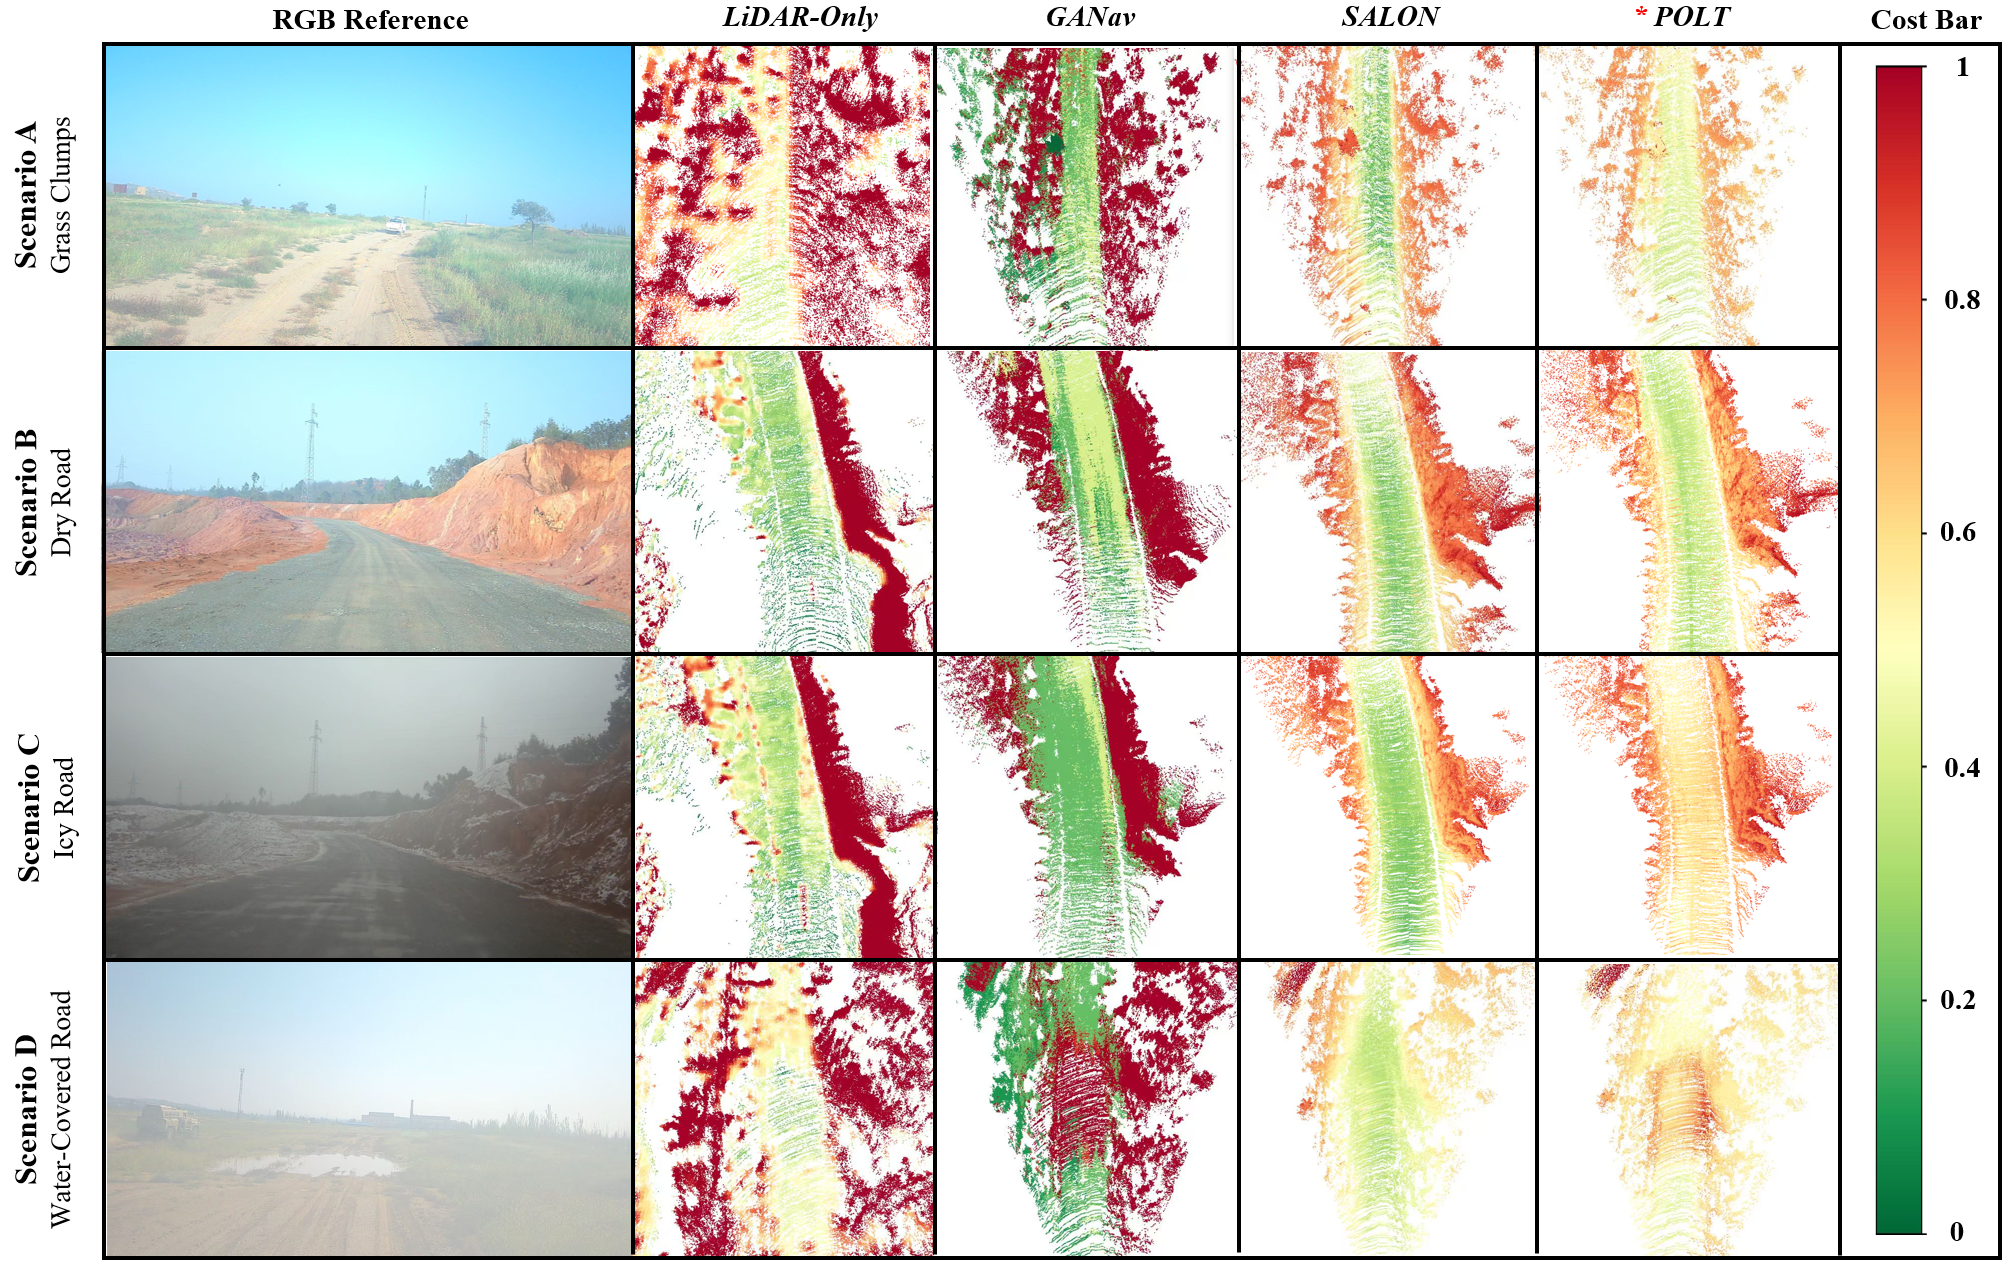
\includegraphics[width=\textwidth]{images/fig_4.png}
    \caption{Qualitative comparison of predicted traversability cost maps across four representative scenarios: (A) Grass clumps causing severe visual occlusion; (B) Dry dirt road; (C) Icy road with slip risk; (D) Waterlogged terrain concealing soft mud. Compared to purely exteroceptive baselines and vertical-only proprioceptive methods (\textit{SALON}), \textit{POLT} demonstrates superior physical consistency. It accurately assigns high costs to tangential hazards (slippery ice and soft mud) while successfully confirming the traversability of deceptive visual obstacles (grass clumps).}
    \label{fig:qualitative_comparison}
\end{figure*}



\section{RESULTS}

\subsection{Experimental Setup}

\textbf{1) Platform:} We employed a wheeled UGV equipped with an RGB camera (Sensing SG2IMX390CH60N), a 128-channel LiDAR (RoboSense RS-Ruby 128), and an INS (StarNeto XWGI7660), while the wheel speeds, steering angles and other chassis data are obtained from the CAN bus. The sensors were synchronized and calibrated, and RGB images, LiDAR point clouds, odometry, IMU measurements, and vehicle chassis states are collected in real-time to facilitate subsequent performance benchmarking and comparative validation.

\textbf{2) Implementation Details:} Details of the proposed method are given as follows to ensure the reproducibility.

\begin{itemize}
\item \textbf{Proprioceptive Model Training:} T-PINN's temporal input window is set to $T_{step}=50$ (1.0 s). The MLP decoder utilizes a hidden structure of [128, 64, 32]. We employ the Adam optimizer (batch size 32, initial learning rate $\eta=10^{-3}$) for $N_{epoch}=200$. To prevent early-stage parameter oscillation, a two-stage warm-up strategy is applied: the first 20 epochs optimize solely the data-driven loss ($\lambda_{data}=1.0$), followed by joint optimization with the Dugoff-based physics ($\lambda_{phy}=0.5$) and state constraint ($\lambda_{state}=0.1$) losses.

\item \textbf{Online Learning Mechanism:} The real-time GPR employs a Matérn kernel ($\nu=0.5$) optimized via L-BFGS to model non-stationary terrain variations. Dynamic memory management is strictly governed by specific thresholds: prediction error difference $\mu_{diff}=0.1$, feature similarity $\epsilon=0.8$, and triggering counts $N_{conflict}=3$ and $N_{merge}=3$ for the conflict and merge mechanisms, respectively. For local mapping, LiDAR point clouds are accumulated over $N_{acc}=100$ historical frames and pre-processed using a voxel grid downsampling filter ($V_{size}=0.2$m) to generate a $0.2$ m/pixel BEV map.
\end{itemize}


\begin{figure}[t]
  \centering
  % 建议文件名不要带空格，如 fig_5.png
  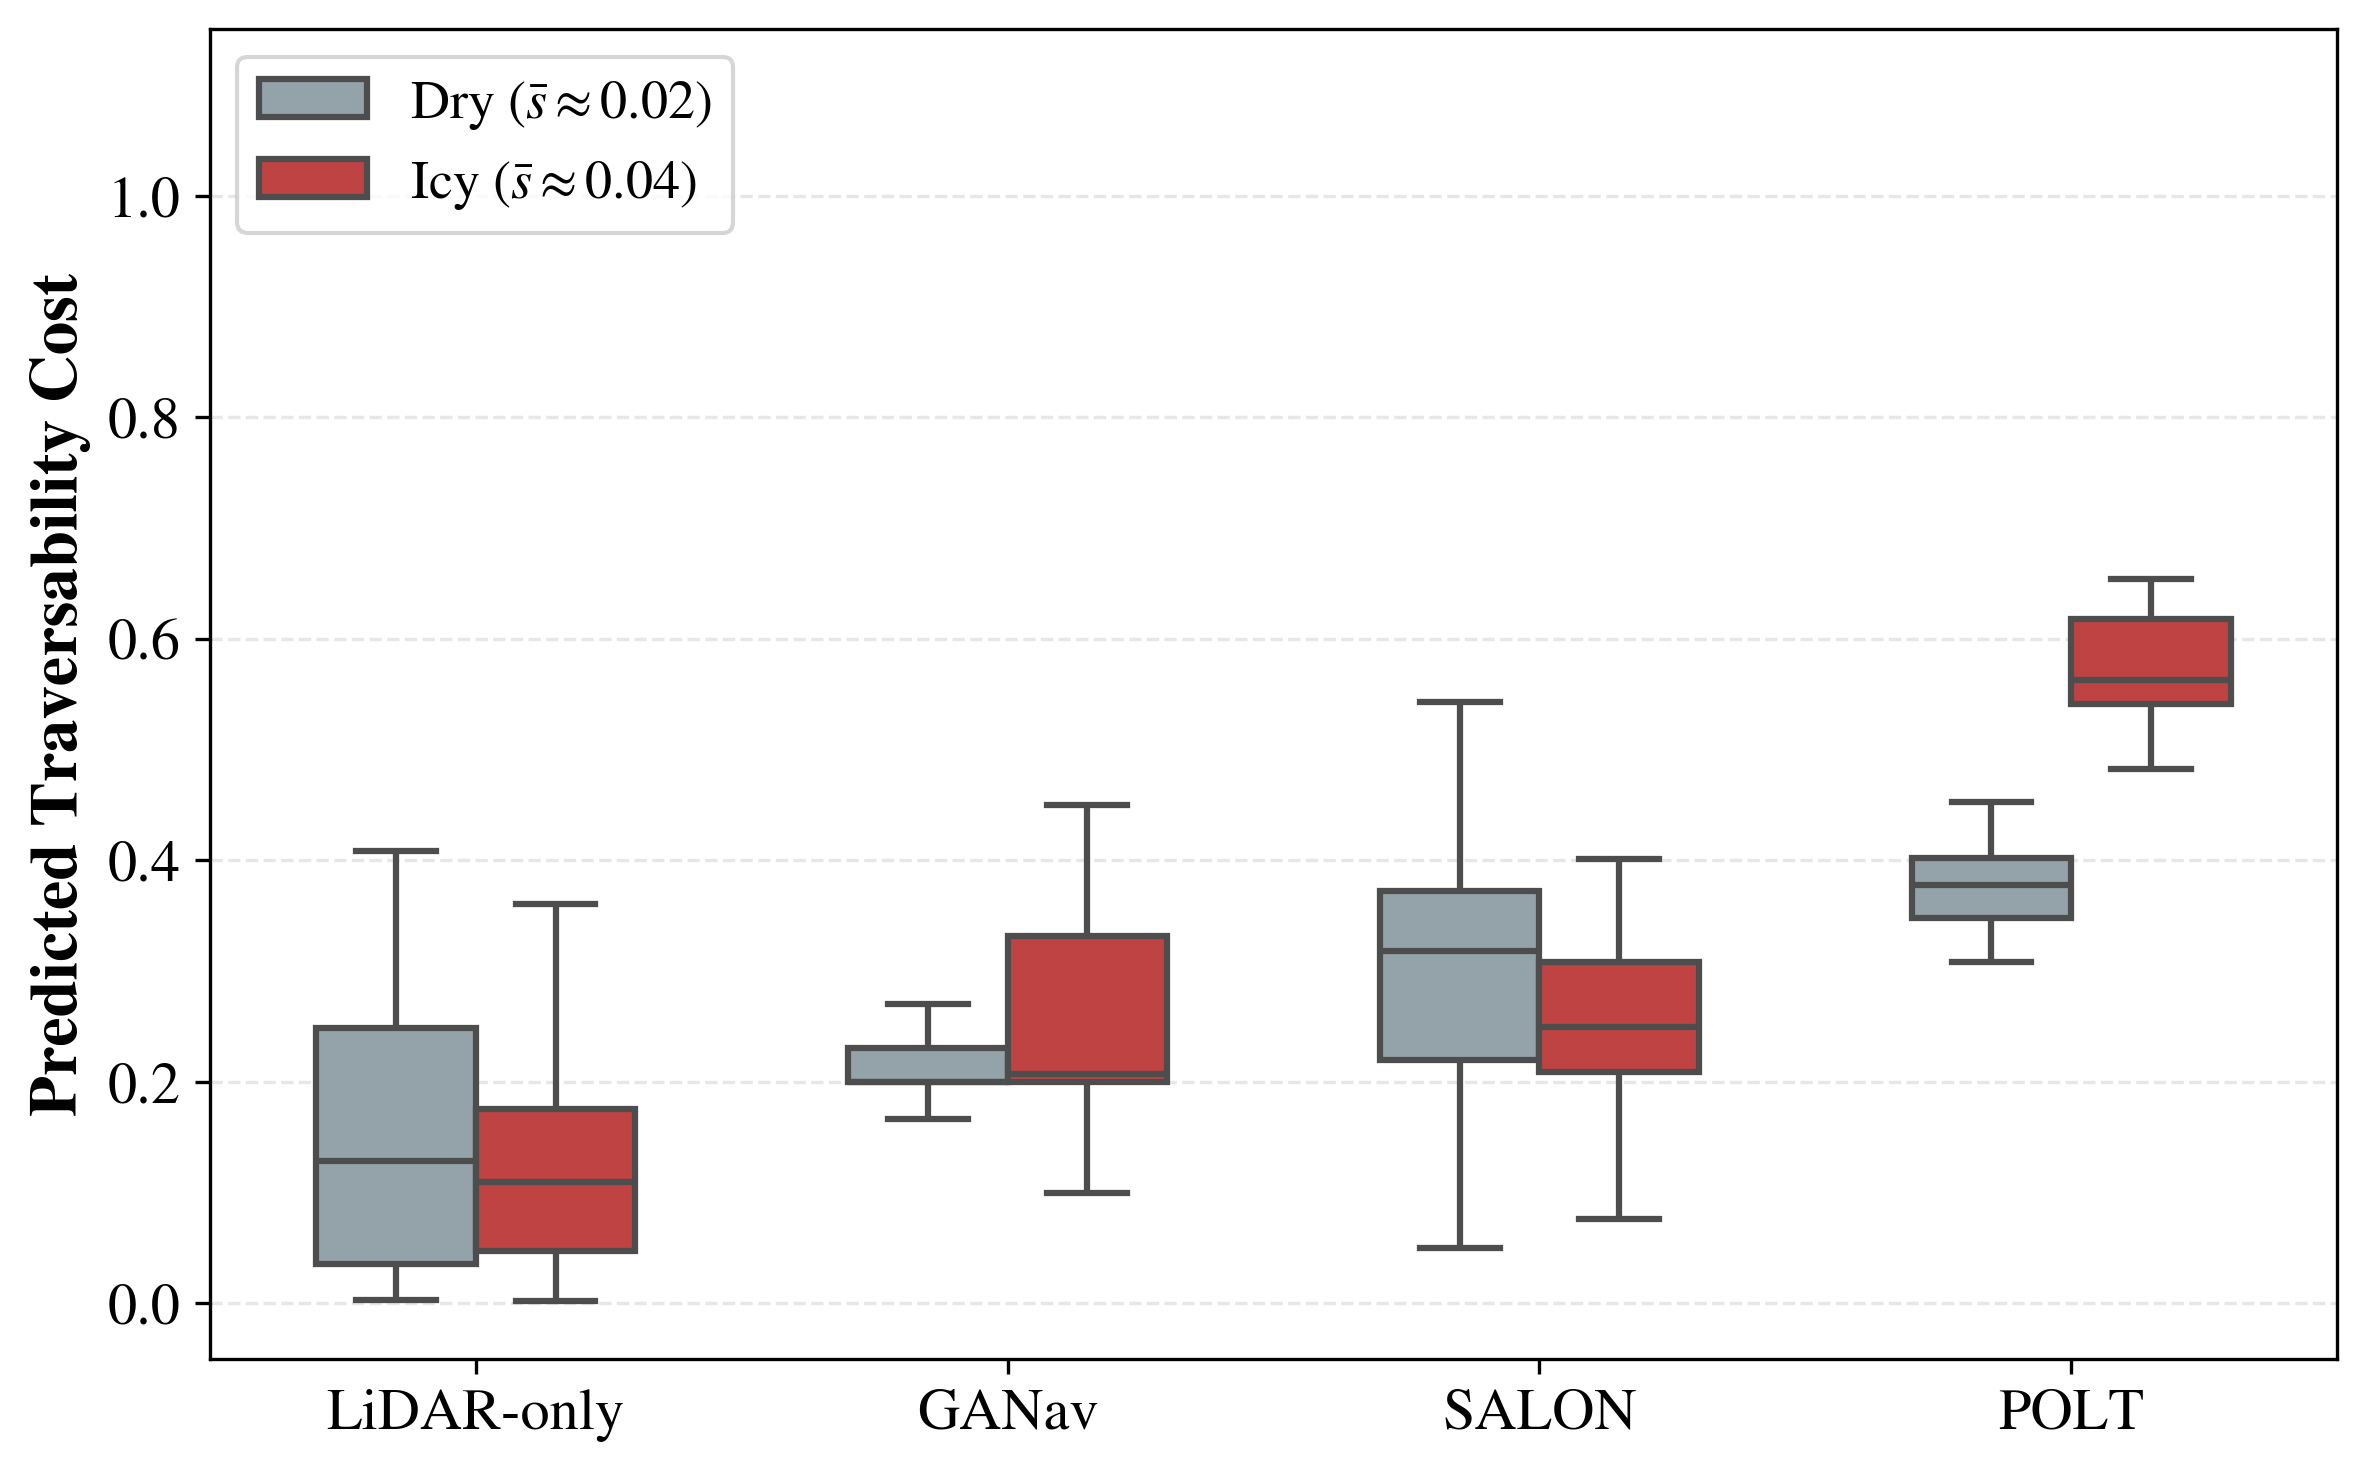
\includegraphics[width=0.48\textwidth]{images/fig_5.png} 
  \caption{Traversability cost distributions under varying friction conditions. The boxplots compare the predicted costs of different methods on dry ($\protect\bar{s} \approx 0.02$) versus icy ($\protect\bar{s} \approx 0.04$) curves. Only \textit{POLT} exhibits a decisive, physically consistent upward shift in the predicted cost on the hazardous icy surface, whereas baseline methods suffer from severe perceptual aliasing.}
  \label{fig:cost_distribution}
\end{figure}

\begin{table}[t]
% \vspace*{2mm} % <--- 加入这行
\centering
\caption{Anomalous Patch Awareness Rate (APAR)}
\label{tab:APAR_comparison}
\resizebox{\columnwidth}{!}{%
\begin{tabular}{l|ccc}
\toprule
\textbf{Methods} & \textbf{Waterlogged} & \textbf{Grass Clumps} & \textbf{Average APAR} \\ 
\midrule
\textbf{\textit{POLT}} & \textbf{100.0\% (12/12)} & \textbf{100.0\% (7/7)} & \textbf{100.0\%} \\ 
\midrule
\textit{SALON} [10]  & 0.0\% (0/12)   & 100.0\% (7/7)   & 36.8\% \\ 
\midrule
\textit{GANav} [18] & 91.67\% (11/12)& 0.0\% (0/7)     & 57.9\% \\
\midrule
\textit{LiDAR-Only} [12]& 0.0\% (0/12)   & 0.0\% (0/7)     & 0.0\% \\ 
\bottomrule
\end{tabular}%
}
\end{table}

\subsection{Comparative Experiments under Multiple Scenarios}


\textbf{1) Baselines:} Three representative baseline methods are selected for comparative experiments, which encompass various surface representation dimensions (geometric and semantic) and distinct learning paradigms (offline and online). The specific baselines are as follows:

\begin{itemize}
\item \textbf{\textit{LiDAR-Only Method} [12]:} This method calculates the traversability cost based on the local elevation variance and geometric distribution of LiDAR point clouds. It represents a classic non-learning, purely geometric approach.
\item \textbf{\textit{GANav} [18]:} An advanced offline visual semantic segmentation method designed for off-road scenarios, representing pure-vision solutions that rely heavily on offline annotated data.
\item \textbf{\textit{SALON} [10]:} An online self-supervised learning method that utilizes a pre-trained visual encoder to extract features and maintains a simple data buffer to regress terrain roughness online.
\end{itemize}



\textbf{2) Qualitative Analysis in Four Representative Scenarios:} Fig. \ref{fig:qualitative_comparison}  illustrates the traversability cost map predictions of the four methods across grass clump-covered, dry, icy/snowy, and waterlogged terrains. The results demonstrate that \textit{POLT} achieves exceptional embodied cognition and scene generalization capabilities:

\begin{itemize}
\item \textbf{Scenario A (Grass Clumps):} Grass clumps cause severe visual occlusion, deceiving \textit{LiDAR-Only} and \textit{GANav} into misclassifying them as rigid obstacles. However, by utilizing proprioceptive feedback, both \textit{POLT} and \textit{SALON} immediately confirm the vegetation's low collision resistance, successfully recalibrating the area into a safely navigable region.

\item \textbf{Scenarios B \& C (Dry vs. Icy/Snowy Terrains):} On icy roads, friction drops while geometry remains flat. \textit{LiDAR-Only} is deceived by the smooth surface, and \textit{GANav} fails on out-of-distribution (OOD) snowy scenes. Crucially, \textit{SALON} misses the slip risk by relying solely on vertical vibration. Conversely, \textit{POLT} captures abnormal tangential wheel-slip states via vehicle dynamics, accurately assigning high traversability costs to avoid slippage.

\item \textbf{Scenario D (Waterlogged Terrains):} Waterlogged terrains often conceal soft mud. \textit{LiDAR-Only} fails over water reflections, and \textit{GANav} unreasonably exaggerates the cost by marking puddles as impassable lakes. Because water damping suppresses vertical impacts, \textit{SALON}’s vibration feedback confuses puddles with firm dirt. In contrast, \textit{POLT} precisely perceives the underlying tangential sinkage risk, assigning a physically consistent medium-high cost.
\end{itemize}



3) \textbf{Quantitative Analysis:} Two experiments were conducted to quantitatively validate the improvement of our method in unknown complex conditions.


\textit{a) Experiment on Varying Road Conditions:} In Fig. \ref{fig:cost_distribution}, the above four methods are tested under two distinct conditions, the dry road and icy road. The average wheel slip ratios $\bar{s}$ are 0.02 and 0.04, respectively, implying that the traversability cost on the latter terrain is supposed to be higher. The figure demonstrates the baseline methods exhibit almost no discriminative capability between the two distinct terrains; conversely, our proposed method demonstrates a distinctly elevated cost in the icy road.

Specifically, the baselines suffer from severe perceptual aliasing. Misled by smooth geometry and slight vibrations, LiDAR-Only and \textit{SALON} erroneously assign lower costs to icy terrains than to dry terrains. Similarly, \textit{GANav} fails to capture mechanical degradation, resulting in low-cost predictions. In contrast, \textit{POLT} leverages vehicle dynamics to accurately detect latent slip risks, predicting a physically consistent, higher cost distribution on icy road.

\textit{b) Experiment on Anomalous Patch Conditions:} To quantify proprioceptive awareness across anomalous environmental boundaries, we evaluate the Anomalous Patch Awareness Rate (APAR) on 12 waterlogged and 7 grass clump sequences. A prediction is deemed successful if the cost margin ($c_{target} - c_{adj}$) between the anomalous patch and adjacent normal terrain reflects actual physical constraints: strictly exceeding 0.2 for hidden hazards (waterlogged) or remaining bounded within 0.2 for traversable occlusions (grass clumps).

As shown in Table I, our method achieves a 100\% average APAR, successfully resolving ambiguities where baselines exhibit severe domain biases. The geometric-based \textit{LiDAR-Only} approach fails completely in both scenarios (0\%); the semantic-based \textit{GANav} identifies water hazards (91.67\%) but fails entirely in grass clumps (0\%) due to rigid visual priors; whereas \textit{SALON} evaluates grass clumps as traversable (100\%) but entirely misses waterlogged mud (0\%), confusing water damping with firm dirt. Our proprioception-based method overcomes both false positives and false negatives, demonstrating robust physical consistency across anomalous terrains.


\begin{figure}[t]
    \centering
    % 子图 (a) - 效率
    \subfloat[Efficiency]{
        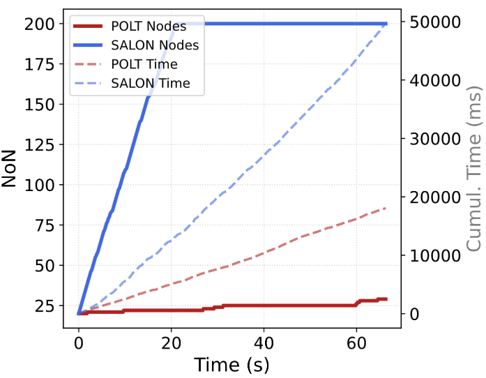
\includegraphics[width=0.47\columnwidth]{images/fig_6a.png} % 建议略微调小至 0.47
        \label{fig:ablation_efficiency}
    }% <-- 注意这里的百分号，用来消除换行带来的空格
    \hfill % 撑开中间间距
    % 子图 (b) - 收敛
    \subfloat[Convergence]{
        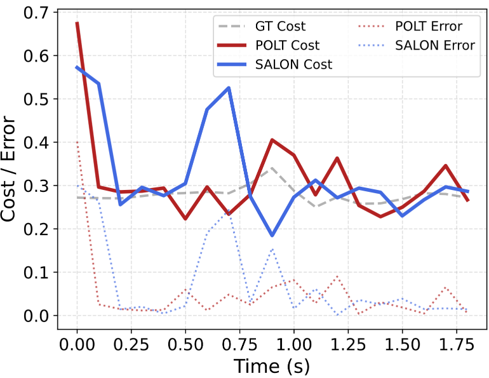
\includegraphics[width=0.47\columnwidth]{images/fig_6b.png}
        \label{fig:ablation_convergence}
    }
    \caption{Ablation study on the memory mechanisms. (a) Computational efficiency comparison. (b) Convergence trajectories of the predicted traversability cost when encountering abrupt terrain transitions. Note: \textit{POLT} and \textit{SALON} denote our dynamic memory and the fixed-size data buffer baseline, respectively.}
    \label{fig:ablation}
\end{figure}

\begin{table}[t]
\vspace*{4mm}
\centering
\caption{Ablation Study on Memory Mechanism Efficiency}
\label{tab:ablation_memory}
\resizebox{\columnwidth}{!}{%
\begin{tabular}{l|ccc}
\toprule
\textbf{Methods} & \textbf{NoN} $\downarrow$ & \textbf{AIT (ms)} $\downarrow$ & \textbf{CT (s)} $\downarrow$ \\ 
\midrule
\textbf{\textit{POLT (Dynamic Memory)}} & \textbf{29} & \textbf{30.05} & \textbf{0.2} \\ 
\midrule
\textit{SALON (Data Buffer)}    & 200 & 82.60 & 1.0 \\
\bottomrule

\end{tabular}%
}
\end{table}

\subsection{Ablation Study}

We validate the efficiency and adaptability of our dynamic memory mechanism by comparing it against the fixed-size data buffer baseline utilized in \textit{SALON}.

\textbf{1) Experimental Design:} We conducted a continuous driving trial comprising two sequential phases. The UGV first operates in Phase 1 (a homogeneous terrain) for 60 seconds to evaluate computational efficiency. This is quantified by the Number of Nodes (NoN), denoting the training data size for GPR, and the Average Inference Time (AIT) per frame. Subsequently, the UGV transitions into Phase 2 (a distinctly different terrain) to test adaptation speed. This is measured by Convergence Time (CT), defined as the time required for the prediction error to drop strictly below 0.1.

\textbf{2) Computational Efficiency:} In Phase 1 (Fig. \ref{fig:ablation}(a) and Table \ref{tab:ablation_memory}), \textit{POLT} restricts the NoN to 29, yielding an AIT of 30.05 ms. In contrast, the \textit{SALON}-based Data Buffer baseline continuously saturates its fixed capacity, leading to a higher AIT of 82.60 ms. This demonstrates that \textit{POLT} significantly reduces the computational burden while maintaining effective representational capacity.

\textbf{3) Rapid Adaptation:} Upon transitioning to Phase 2 (Fig. \ref{fig:ablation}(b)), the \textit{SALON}-based Data Buffer baseline exhibits a perceptual hysteresis of 1.0 s. Conversely, by executing conflict correction, concept reinforcement, and incremental updates, \textit{POLT} rapidly adapts to the new terrain features. As summarized in Table \ref{tab:ablation_memory}, it achieves accurate predictions with a CT of 0.2 s, demonstrating strong self-adaptive capabilities.


\section{CONCLUSIONS}

In this work, we present \textit{POLT}, an embodied traversability prediction method designed to address the critical vision-mechanics ambiguity in complex terrains. By establishing a unified exteroception-proprioception-memory paradigm, we utilize a physics-informed T-PINN to learn traversability cost from noisy proprioceptive feedback. Additionally, a GPR-based dynamic memory seamlessly integrates offline priors with online experiences, effectively bridging the gap between visual appearance and physical reality. Real-world experiments confirm that \textit{POLT} robustly outperforms existing baselines in complex terrains. Future work will focus on investigating the generalizability of the proposed T-PINN proprioceptive framework across diverse platforms with varying dynamics and vehicle parameters, as well as extending its application to a broader range of complex scenarios.


% \addtolength{\textheight}{-12cm}   % This command serves to balance the column lengths
                                  % on the last page of the document manually. It shortens
                                  % the textheight of the last page by a suitable amount.
                                  % This command does not take effect until the next page
                                  % so it should come on the page before the last. Make
                                  % sure that you do not shorten the textheight too much.


% \addtolength{\textheight}{-2cm} % 这里的数值需根据实际留白量微调，例如从-1cm试到-15cm

\begin{thebibliography}{99}

\bibitem{c1} J. Behley, M. Garbade, A. Milioto, J. Quenzel, S. Behnke, C. Stachniss, and J. Gall, SemanticKITTI: A dataset for semantic scene understanding of LiDAR sequences, in Proc. IEEE/CVF Int. Conf. Comput. Vis. (ICCV), 2019.

\bibitem{c2} T. Shan, B. Englot, D. Meyers, W. Wang, C. Ratti, and D. Rus, LIO-SAM: Tightly-coupled lidar inertial odometry via smoothing and mapping, in Proc. IEEE/RSJ Int. Conf. Intell. Robots Syst. (IROS), 2020.

\bibitem{c3} P. Papadakis, Terrain traversability analysis methods for unmanned ground vehicles: A survey, Eng. Appl. Artif. Intell., 2013.

\bibitem{c4} G. Kahn, P. Abbeel, and S. Levine, BADGR: An autonomous self-supervised learning-based navigation system, IEEE Robot. Autom. Lett., 2021.

\bibitem{c5} C. C. MacAdam, Understanding and modeling the human driver, Veh. Syst. Dyn., 2003.

\bibitem{c6} R. O. Chavez-Garcia and O. Aycard, Multiple sensor fusion and classification for moving object detection and tracking, IEEE Trans. Intell. Transp. Syst., 2015.

\bibitem{c7} M. G. Castro, S. Triest, W. Wang, J. M. Gregory, F. Sanchez, J. G. Rogers, and S. Scherer, How does it feel? Self-supervised costmap learning for off-road vehicle traversability, in Proc. IEEE Int. Conf. Robot. Autom. (ICRA), 2023.

\bibitem{c8} L. Wellhausen, A. Dosovitskiy, R. Ranftl, K. Walas, C. Cadena, and M. Hutter, Where should I walk? Predicting terrain properties from images via self-supervised learning, IEEE Robot. Autom. Lett., 2019.

\bibitem{c9} A. Pokhrel, M. Nazeri, A. Datar, and X. Xiao, CAHSOR: Competence-aware high-speed off-road ground navigation in SE(3), IEEE Robot. Autom. Lett., vol. 9, no. 11, pp. 9653--9660, 2024.

\bibitem{c10} M. Sivaprakasam, S. Triest, C. Ho, S. Aich, J. Lew, I. Adu, W. Wang, and S. Scherer, SALON: Self-supervised adaptive learning for off-road navigation, in Proc. IEEE Int. Conf. Robot. Autom. (ICRA), 2025, pp. 16999--17006.

\bibitem{c11} K. Iagnemma and S. Dubowsky, Online terrain parameter estimation for wheeled mobile robots with application to planetary rovers, IEEE Trans. Robot., 2004.

\bibitem{c12} H. Xue, H. Fu, L. Xiao, Y. Fan, D. Zhao, and B. Dai, Traversability analysis for autonomous driving in complex environment: A LiDAR-based terrain modeling approach, IEEE Trans. Intell. Veh. (TIV), 2024.

\bibitem{c13} H. Xie, X. Zhong, B. Chen, P. Peng, H. Hu, and Q. Liu, Real-time elevation mapping with Bayesian ground filling and traversability analysis for UGV navigation, in Proc. IEEE/RSJ Int. Conf. Intell. Robots Syst. (IROS), 2023, pp. 7218--7225.

\bibitem{c14} H. Xue, H. Fu, R. Ren, Y. Zhang, and J. Wang, Lidar-based drivable region detection for autonomous driving, in Proc. IEEE/RSJ Int. Conf. Intell. Robots Syst. (IROS), 2021, pp. 1110--1116.

\bibitem{c15} S. Triest, M. Sivaprakasam, S. Aich, D. Fan, W. Wang, and S. Scherer, Velociraptor: Leveraging visual foundation models for label-free, risk-aware off-road navigation, in Proc. Conf. Robot Learn. (CoRL), 2024.

\bibitem{c16} M. A.-M. Khan, D. Pushp, and L. Liu, AFRDA: Attentive feature refinement for domain adaptive semantic segmentation, IEEE Robot. Autom. Lett., 2025.

\bibitem{c17} M. Ye, Y. Zhang, J. Gu, S. Xiang, L. Kong, and A. Xie, Surface roughness estimation for terrain perception, in Proc. IEEE Int. Conf. Robot. Autom. (ICRA), 2025.

\bibitem{c18} T. Guan, L. Zhang, J. Lin, R. Song, and D. Manocha, GA-Nav: Efficient terrain segmentation for robot navigation in unstructured outdoor environments, IEEE Robot. Autom. Lett., vol. 7, no. 3, pp. 8138--8145, 2022.

\bibitem{c19} F. Ruetz, N. Lawrance, E. Hernández, and T. Peynot, Autonomous hiking trail navigation via semantic segmentation and geometric analysis, in Proc. IEEE/RSJ Int. Conf. Intell. Robots Syst. (IROS), 2025, pp. 52--58.

\bibitem{c20} H. Shon, J. Jeong, and S. Kim, Real-time terrain traversability analysis and mapping for autonomous robotics in dynamic environments: Fusing appearance- and geometry-based approaches, J. Field Robot., 2025.

\bibitem{c21} N. Hanson, M. Shaham, D. Erdogmus, and T. Padir, VAST: Visual and spectral terrain classification in unstructured multi-class environments, in Proc. IEEE/RSJ Int. Conf. Intell. Robots Syst. (IROS), 2022.

\bibitem{c22} C. Yao, F. Xue, Z. Wang, Y. Yuan, Z. Zhu, L. Ding, and Z. Jia, Wheel vision: Wheel-terrain interaction measurement and analysis using a sensorized transparent wheel on deformable terrains, IEEE Robot. Autom. Lett., vol. 8, no. 1, 2023.

\bibitem{c23} F. J. Comin and C. M. Saaj, Models for slip estimation and soft terrain characterization with multilegged wheel–leg, Sensors, vol. 19, no. 14, p. 3030, 2019.

\bibitem{c24} H. Lin, H. Li, and Y. Gao, See-touch-predict: Active exploration and online perception of terrain physics with legged robots, IEEE Robot. Autom. Lett., vol. 10, 2025.

\bibitem{c25} T. Yang and G. Liu, Pressing and rubbing: Physics-informed features facilitate haptic terrain classification for legged robots, IEEE Robot. Autom. Lett., vol. 7, no. 2, pp. 826--833, 2022.

\bibitem{c26} A. H. Chang, C. Hubicki, A. Ames, and P. A. Vela, Every hop is an opportunity: Quickly classifying and adapting to terrain during targeted hopping, in Proc. IEEE Int. Conf. Robot. Autom. (ICRA), 2019, pp. 3188--3194.

\bibitem{c27} M. Prágr, J. Bayer, and J. Faigl, On predicting terrain changes induced by mobile robot traversal, in Proc. IEEE/RSJ Int. Conf. Intell. Robots Syst. (IROS), 2024.

\bibitem{c28} H. Shon, S. Choi, and K. Huh, Real-time terrain condition detection for off-road driving based on transformer, IEEE Trans. Intell. Transp. Syst., vol. 25, 2024.

\bibitem{c29} E. Chen, C. Ho, M. Maulimov, C. Wang, and S. Scherer, RCA: Ride comfort-aware visual navigation via self-supervised learning, in Proc. IEEE/RSJ Int. Conf. Intell. Robots Syst. (IROS), 2022.

\bibitem{c30} C. Brooks and K. Iagnemma, Frequency response method for terrain classification in autonomous ground vehicles, Auton. Robots, vol. 25, pp. 1--15, 2008.

\bibitem{c31} Y. Wang, Y. Zhang, Y. Wang, and Z. Meng, Terrain classification using intelligent tire, J. Terramechanics, vol. 72, pp. 1--12, 2017.

\bibitem{c32} Y. Li, B. Zhu, J. Zhao, and Y. Liu, Terrain classification method based on fusion of vision and vehicle dynamics for UGV, Expert Syst. Appl., vol. 279, p. 127495, 2025.

\bibitem{c33} Y. Bu, Z. Sun, X. Li, J. Zeng, X. Zhang, and H. Shen, Self-supervised traversability learning with online prototype adaptation for off-road autonomous driving, IEEE Robot. Autom. Lett., vol. 10, no. 11, 2025.

\bibitem{c34} E. Chen, C. Ho, M. Maulimov, C. Wang, and S. Scherer, Learning-on-the-drive: Self-supervised adaptive long-range perception for high-speed offroad driving, in Proc. IEEE/RSJ Int. Conf. Intell. Robots Syst. (IROS), 2024.

\bibitem{c35} E. S. Lupu, F. Xie, J. Preiss, and S. Chung, Learning self-supervised traversability with navigation experiences of mobile robots: A risk-aware self-training approach, IEEE Robot. Autom. Lett., 2024.

\bibitem{c36} W. Wang, T. Guan, J. Lin, and D. Manocha, TerraPN: Unstructured terrain navigation using online self-supervised learning, in Proc. IEEE/RSJ Int. Conf. Intell. Robots Syst. (IROS), 2022.

\bibitem{c37} Y. Jeon, E. I. Son, and S. W. Seo, Follow the footprints: Self-supervised traversability estimation for off-road vehicle navigation based on geometric and visual cues, in Proc. IEEE Int. Conf. Robot. Autom. (ICRA), 2024.

\bibitem{c38} A. Rezazadeh, Z. Li, W. Wei, and Y. Bao, From isolated conversations to hierarchical schemas: Dynamic tree memory representation for LLMs, in Proc. Int. Conf. Learn. Represent. (ICLR), 2024.

\bibitem{c39} Z. Zhang, Q. Dai, X. Chen, R. Li, Z. Li, and Z. Dong, MemEngine: A unified and modular library for developing advanced memory of LLM-based agents, in Companion Proc. ACM Web Conf. (WWW), 2025.

\bibitem{c40} W. Zhong, L. Guo, Y. Wang, and Y. Wang, MemoryBank: Enhancing large language models with long-term memory, in Proc. AAAI Conf. Artif. Intell. (AAAI), 2024.

\bibitem{c41} O. Siméoni, M. Oquab, T. Darcet, M. Assran, P. Bojanowski, A. Joulin, and I. Misra, DINOv3: Self-supervised learning for vision at unprecedented scale, arXiv preprint arXiv:2508.00000, 2025.

\end{thebibliography}



\end{document}
